\documentclass[11pt]{article}
\usepackage[margin=0.82in]{geometry}
\usepackage{amsmath,amssymb,booktabs,array,graphicx,xcolor}
\usepackage[colorlinks=true,linkcolor=blue,urlcolor=blue]{hyperref}
\usepackage[T1]{fontenc}
\usepackage{lmodern}
\definecolor{ink}{HTML}{14263D}
\definecolor{accent}{HTML}{2864C7}
\hypersetup{pdftitle={Failure-driven parameter repair: the Kimi implementation},pdfauthor={FailureIsAllYouNeed}}
\setlength{\parindent}{0pt}
\setlength{\parskip}{6pt}
\setlength{\emergencystretch}{2em}
\newcommand{\R}{\mathbb{R}}
\newcommand{\norm}[1]{\left\lVert#1\right\rVert}
\newcommand{\diag}{\operatorname{diag}}
\newcommand{\argmax}{\operatorname*{arg\,max}}
\newcommand{\code}[1]{\texttt{\detokenize{#1}}}
\newcommand{\source}[2]{\href{https://github.com/HarleyCoops/KimiBrainSurgery/blob/13cfaec9f484a1a8864349a814bfd62905022a05/#1}{\nolinkurl{#1}}: #2}
\begin{document}
{\color{accent}\small FAILURE IS ALL YOU NEED \quad / \quad METHODS NOTE}
\begin{center}
{\LARGE\bfseries\color{ink} Failure-driven parameter repair}\par\vspace{8pt}
{\large The equations behind the Kimi implementation}\par\vspace{6pt}
{\small Code-grounded mathematical companion \quad November 3, 2026}
\end{center}

\textbf{Purpose.} Translate the implemented solvers in
\href{https://github.com/HarleyCoops/KimiBrainSurgery}{KimiBrainSurgery}
into explicit objectives, constraints, and parameter updates. This document is
an analysis of saved code and results, not a newly executed repair experiment.
It provides a common mathematical interface for eventually combining Kimi's
analytic solvers with the separate LLM-proposed repair in FailureIsAllYouNeed.

\textbf{Source snapshot.} All implementation claims refer to commit
\begin{center}\small\code{13cfaec9f484a1a8864349a814bfd62905022a05}.\end{center}
Run records were checked through the W\&B MCP connection against
\href{https://forge.coreweave.com/wandb/christian-cooper-us/kimi-brain-surgery}{the Kimi Brain Surgery project}:
18 sweep runs, one monotonic run, and one paired-evaluation run.
The repository includes copied numerical records and their source hashes.

\textbf{The central operation.} Given a failed decision, choose an update that
increases a saving action's logit relative to the wrong action while penalizing
changes on other observations. The basic subproblem is
\begin{equation}
 \min_{\delta}\;\frac12\delta^{\mathsf T}M\delta
 \quad\text{subject to}\quad a^{\mathsf T}\delta=t,
 \qquad
 \delta^*=\frac{t\,M^{-1}a}{a^{\mathsf T}M^{-1}a}.
 \label{eq:master}
\end{equation}
Here $a$ describes sensitivity of the target decision, $M$ penalizes edit size
and interference, and $t$ is the required logit-gap correction.
The formula requires $M\succ0$ and $a\ne0$.

\textbf{What is exact, and what is local?}
\begin{center}
\begin{tabular}{p{0.22\linewidth}p{0.69\linewidth}}
\toprule
Method & Mathematical status \\
\midrule
Readout $W_3$ & Hidden activations stay fixed. The selected pair's logit-gap change is exact. \\
Rank-one $W_2$ & Exact preactivation change followed by a first-order approximation through $\tanh$. \\
Unrestricted $W_2$ & The same local approximation with all $32\times32$ entries available, solved in blocks. \\
Keep/rollback & Nondecreasing mean return on the reused 64-game gate, by construction. No global guarantee. \\
\bottomrule
\end{tabular}
\end{center}

\textbf{Interpretation.} This is constrained inverse behavior design. It is not
an inverse of the original training trajectory. The $W_2$ solvers explicitly
use analytic derivatives; they do not run a gradient-descent training loop.
Kimi's language-model weights are not being modified. The edited object is a
small, previously PPO-trained game policy.

\clearpage
\normalsize
\section{Policy, failure signal, and diagnosis}
Use column vectors; the source uses equivalent row-vector NumPy expressions.
For a flattened one-hot grid observation $x\in\R^{500}$,
\begin{align}
 u(x)&=\tanh(W_1^{\mathsf T}x+b_1)\in\R^{32},\nonumber\\
 z(x)&=W_2^{\mathsf T}u(x)+b_2,\qquad h(x)=\tanh z(x)\in\R^{32},\nonumber\\
 \ell(x)&=W_3^{\mathsf T}h(x)+b_3\in\R^5,\qquad
 \pi(x)=\argmax_{c}\ell_c(x).
 \label{eq:network}
\end{align}
Shapes are $W_1:500\times32$, $W_2:32\times32$, $W_3:32\times5$;
bias lengths are 32, 32, and 5. Total: 17,253 parameters.
Actions 0, 1, and 2 leave the paddle still; 3 moves left and 4 moves right.

\subsection*{From a trajectory to an avoidable decision}
The miner predicts the next ball contact column $c_*$ and the number $T$ of
remaining ticks. For current paddle center $p$, let
$p_c=\operatorname{clip}(p+\mathrm{move}(c),2,7)$.
After that action, the paddle centers reachable before contact form
\begin{equation}
 I_c=[\max(2,p_c-(T-1)),\ \min(7,p_c+(T-1))].
\end{equation}
A width-three paddle can still intercept the ball if
$I_c\cap[c_*-1,c_*+1]\ne\varnothing$.
The saving set $S_f$ contains the canonical actions $\{0,3,4\}$ satisfying this
test. A failure is recorded when the chosen action destroys this reachability
and $S_f$ is nonempty. A saving action preserves an available route to contact;
it does not guarantee that the edited policy will choose that route later.

The original miner considers descending balls only. Its landing predictor is
a simplified descent calculation and aborts on a predicted diagonal brick hit.
The later \code{use_flight=True} path simulates ascent, wall and brick collisions,
and brick removals until the next paddle-row arrival, with a 1,000-tick cap.
It mirrors the simulator's ball physics. This exposes failures to pre-position
the paddle during ascent that the original miner cannot see.

Default mining uses seeds 0--199 and at most 200 steps per game. Every visited
observation becomes a probe; failures are deduplicated by observation bytes.
The outer loop selects the first eligible failure.

\subsection*{Which logit contributions favor the wrong action?}
At failure $x_f$, set $a=\pi(x_f)$ and
$b=\argmax_{c\in S_f}\ell_c(x_f)$. The initial wrong-minus-saving gap is
\begin{equation}
 g=\ell_a(x_f)-\ell_b(x_f)
  =\sum_{j=1}^{32}h_{f,j}(W_{3,ja}-W_{3,jb})+(b_{3,a}-b_{3,b}).
 \label{eq:gap}
\end{equation}
The diagnostic sorts the hidden-unit summands and reports the three largest.
The bias term is part of the exact gap but is absent from that ranked list.
This decomposition explains the current logits; it does not identify a unique
causal parameter subset or imply that only three units will be edited.

\small Source: \source{failure_gym.py}{\code{mine}, \code{flight_landing}, \code{diagnose}};
\source{assets/policy.py}{forward pass and action selection}.

\clearpage
\normalsize
\section{Exact readout edits: naive and probe-protected \texorpdfstring{$W_3$}{W3}}
Let $m>0$ be the desired pairwise margin ($m=0.1$ by default) and $t=g+m$.
Only two output columns change:
\begin{equation}
 \Delta W_3[:,a]=-\tfrac12d,\qquad
 \Delta W_3[:,b]=+\tfrac12d,\qquad \Delta b_3=0.
 \label{eq:w3columns}
\end{equation}
Since $h_f$ is unchanged, $g_{\mathrm{new}}=g-h_f^{\mathsf T}d$ exactly.
Enforcing $h_f^{\mathsf T}d=t$ therefore gives
$\ell_b^{\mathrm{new}}-\ell_a^{\mathrm{new}}=m$.
Other action logits can still exceed $\ell_b^{\mathrm{new}}$: the gate separately
checks whether the global argmax belongs to $S_f$.

The minimum-size update without probe protection is
\begin{equation}
 \min_d\norm{d}_2^2\ \text{s.t.}\ h_f^{\mathsf T}d=t
 \quad\Longrightarrow\quad d=\frac{t}{\norm{h_f}_2^2}h_f.
\end{equation}
It changes up to 64 scalar entries, not one isolated weight.

\subsection*{A soft preservation penalty}
Stack current probe hidden activations as rows of $H\in\R^{N\times32}$.
The implemented protected edit solves
\begin{align}
 \min_d\quad &\norm{d}_2^2+\frac{\lambda}{N}\norm{Hd}_2^2,
 &\text{s.t.}\quad h_f^{\mathsf T}d=t,\nonumber\\
 M&=I+\frac{\lambda}{N}H^{\mathsf T}H,
 &d^*&=\frac{t\,M^{-1}h_f}{h_f^{\mathsf T}M^{-1}h_f}.
 \label{eq:w3}
\end{align}
Under the symmetric update, $\norm{\Delta W_3}_F^2=\norm{d}_2^2/2$ and
the total squared movement of the two affected probe logits is
$\norm{Hd}_2^2/2$. The objective therefore balances parameter size and exact
probe-logit interference, up to a common factor.

\subsection*{Derivation of the common solver}
For Equation~\eqref{eq:master}, write
$L(\delta,\eta)=\tfrac12\delta^{\mathsf T}M\delta
-\eta(a^{\mathsf T}\delta-t)$.
Stationarity gives $M\delta=\eta a$; substitution into the constraint gives
$\eta=t/(a^{\mathsf T}M^{-1}a)$. The implementation uses a linear solve,
not an explicit matrix inverse.

\subsection*{What ``null-space'' means here}
At finite $\lambda$, Equation~\eqref{eq:w3} is a soft quadratic penalty,
not the hard condition $Hd=0$. Larger $\lambda$ favors directions that disturb
the sampled probes less, but can increase edit size. Exact preservation and a
nonzero target are jointly possible only if $h_f$ has a nonzero component in
$\ker H$. If $H$ has full column rank, there is no nonzero exact null-space edit.

The probe subsampling stride is $\max(1,\lfloor P/4000\rfloor)$ for $P$ probes;
4,000 is a target, not a strict sample cap. $N$ in the equations is the actual
number selected. Probes are regenerated from each current policy.

\small Source: \source{failure_gym.py}{\code{solve}};
\source{nullspace_gym.py}{\code{solve_constrained}}.

\clearpage
\normalsize
\section{Rank-one \texorpdfstring{$W_2$}{W2} repair through a nonlinearity}
Keep $W_1$, $W_3$, and all biases fixed. Restrict the update to
\begin{equation}
 \Delta W_2=u_fv^{\mathsf T},\qquad v\in\R^{32}.
\end{equation}
For any probe $p$, its preactivation change is exact:
\begin{equation}
 \Delta z_p=(\Delta W_2)^{\mathsf T}u_p=(u_p^{\mathsf T}u_f)v.
\end{equation}
Define $D_p=\diag(1-h_p\odot h_p)$. The hidden change has the local expansion
\begin{equation}
 \Delta h_p=D_p\Delta z_p+O(\norm{\Delta z_p}^2).
 \label{eq:tanh}
\end{equation}
Let $w=W_3[:,b]-W_3[:,a]$ be the saving-minus-wrong readout direction.
At the failure, the linearized improvement in that logit difference is
\begin{equation}
 w^{\mathsf T}\Delta h_f\ \simeq\
 \norm{u_f}_2^2 w^{\mathsf T}D_fv=a_f^{\mathsf T}v,
 \qquad a_f=\norm{u_f}_2^2D_fw.
\end{equation}
Thus the local target is $a_f^{\mathsf T}v=t=g+m$.

\subsection*{Implemented objective and diagonal solve}
With $c_p=(u_p^{\mathsf T}u_f)^2$, the subproblem is
\begin{equation}
 \min_v\;\mu\norm{v}_2^2+
 \frac{\lambda}{N}\sum_{p=1}^N c_p\norm{D_pv}_2^2
 \quad\text{s.t.}\quad a_f^{\mathsf T}v=t.
\end{equation}
Its metric is diagonal:
\begin{align}
 A_j&=\mu+\frac{\lambda}{N}\sum_{p=1}^N
       (u_p^{\mathsf T}u_f)^2(1-h_{p,j}^2)^2,\nonumber\\
 v_j^*&=\frac{t\,(a_{f,j}/A_j)}{\sum_k a_{f,k}^2/A_k},
 \qquad \Delta W_2=u_f(v^*)^{\mathsf T}.
 \label{eq:rankone}
\end{align}
The source sets $\mu=1$. Its regularizer is $\norm{v}^2$, whereas
$\norm{\Delta W_2}_F^2=\norm{u_f}^2\norm{v}^2$.
The probe term protects first-order hidden activations, not directly return
or even all logit margins. Small activation movement can still flip a close
argmax decision.

\subsection*{Sequential local corrections}
The code takes at most eight inner steps. It recomputes the actual failure
logits, $g$, $h_f$, and $D_f$ each step. It stops as soon as the global greedy
action is in $S_f$; this stopping rule need not attain margin $m$.
The probe activations and derivatives are computed once before the inner loop
and stay frozen during its corrections. The initial $a$ and $b$ action indices
also stay fixed. $u_f$ stays fixed because $W_1$ is unchanged.

Each proposed step is rescaled to Frobenius norm at most 1 before application.
After clipping, even its linearized equality need no longer hold. The source
calls these ``Newton'' steps; they are sequential local gap corrections, not
an exact Newton method for the full nonlinear return objective.

\small Source: \source{w2_gym.py}{\code{solve_w2}, \code{probe_stats}}.

\clearpage
\normalsize
\section{Unrestricted \texorpdfstring{$W_2$}{W2}: a block-diagonal quadratic solve}
Now allow any $\Delta\in\R^{32\times32}$, with columns $\delta_j$.
``Full-rank'' names this unrestricted parameterization; the computed update
need not have matrix rank 32.
For a probe, $\Delta z_p=\Delta^{\mathsf T}u_p$ exactly and
$\Delta h_p\simeq D_p\Delta^{\mathsf T}u_p$ locally.
The implementation minimizes
\begin{equation}
 \mathcal{C}(\Delta)=\mu\norm{\Delta}_F^2+
 \frac{\lambda}{N}\sum_p\norm{D_p\Delta^{\mathsf T}u_p}_2^2.
 \label{eq:fullobjective}
\end{equation}
Because the hidden-activation norm sums over units without cross-unit terms,
\begin{align}
 G_j&=\frac1N\sum_p (1-h_{p,j}^2)^2u_pu_p^{\mathsf T},\nonumber\\
 \mathcal{C}(\Delta)&=\sum_{j=1}^{32}\delta_j^{\mathsf T}M_j\delta_j,
 \qquad M_j=\mu I+\lambda G_j.
\end{align}
The saving-minus-wrong constraint becomes
\begin{equation}
 \sum_j a_j^{\mathsf T}\delta_j=t,
 \qquad a_j=(D_fw)_j u_f.
 \label{eq:fullconstraint}
\end{equation}
Stacking columns would produce a 1,024-dimensional vector and a block-diagonal
metric. Instead, solve 32 small systems:
\begin{equation}
 y_j=M_j^{-1}a_j,
 \qquad s=\sum_k a_k^{\mathsf T}y_k,
 \qquad \boxed{\delta_j^*=\frac{t}{s}y_j}.
 \label{eq:fullsolution}
\end{equation}
This is Equation~\eqref{eq:master} applied to the stacked vector. It avoids
a dense $1024\times1024$ inverse. The block structure is a consequence of the
chosen hidden-state penalty; a full logit-preservation penalty can introduce
couplings between blocks through $W_3$.

\subsection*{Exact implementation order}
\begin{enumerate}
\item Select a strided subset of the current probes. Compute $u_p,D_p,G_j$ once.
\item At the current failure state, recompute $g,D_f$ and the actual greedy action.
      Stop if that action belongs to $S_f$.
\item Set $t=g+0.1$, form $a_j$, and solve Equation~\eqref{eq:fullsolution}
      with $\mu=1$.
\item Rescale $\Delta\leftarrow\Delta\min(1,1/\norm{\Delta}_F)$ if nonzero,
      then apply $W_2\leftarrow W_2+\Delta$.
\item Repeat steps 2--4 up to eight corrections. Recompute the probe geometry
      only when the next outer repair starts.
\end{enumerate}

\textbf{Feasibility and numerical limits.} For $\lambda\ge0$ and $\mu>0$, each
$M_j$ is positive definite. The denominator $s$ is positive only if the
constraint sensitivity is nonzero. Saturation, a zero feature vector, or equal
readout columns can make the local target infeasible. The pinned solvers do not
explicitly guard all zero-denominator cases. Float64 local diagnostics and
float32 rollout evaluation also need not make identical near-tie decisions.

\small Source: \source{fullrank_gym.py}{\code{solve_fullrank}};
\source{chase_unresolved.py}{same structure with configurable margin}.

\clearpage
\normalsize
\section{Measurement, composition, and the keep/rollback rule}
For a fixed gate set $G$ of 64 seeds (10000--10063), let
\begin{equation}
 \widehat J_G(\theta)=\frac1{|G|}\sum_{s\in G}R(\theta,s).
\end{equation}
Rollouts use greedy actions, float32 weights, and a 200-step horizon.
The reported probe-flip fraction is
\begin{equation}
 F_P(\theta,\theta')=\frac1{|P|}\sum_{x\in P}
 \mathbf1\{\pi_\theta(x)\ne\pi_{\theta'}(x)\}.
\end{equation}
The \code{fixed} field checks only whether $\pi_{\theta'}(x_f)\in S_f$ at the
stored observation. It does not replay the full failed trajectory or establish
that the edited policy still visits that observation.

\subsection*{The 18 sweep runs are not monotonic loops}
Each of the three solver families sweeps
$\lambda\in\{0,1,10,100,1000,10000\}$ for up to eight outer repairs.
The sweep code assigns \code{weights = new_weights} unconditionally after each
measurement, including failed local fixes and return regressions. Its ``gate''
is a measurement battery, not a promotion filter. These curves reveal edit
interference and composition; they are not sequences of accepted improvements.

\subsection*{The separate monotonic loop}
For a candidate $\widetilde\theta_k$, the actual implemented update is
\begin{equation}
 \theta_{k+1}=\begin{cases}
 \widetilde\theta_k,&\widehat J_G(\widetilde\theta_k)\ge\widehat J_G(\theta_k),\\
 \theta_k,&\text{otherwise}.
 \end{cases}
 \label{eq:gate}
\end{equation}
Consequently $\widehat J_G(\theta_{k+1})\ge\widehat J_G(\theta_k)$.
This is monotonicity of a finite, repeatedly consulted mean. It does not imply
monotonic return on each gate seed or on any unseen distribution.

The rule does \emph{not} additionally require \code{fixed=True}, a maximum
probe-flip rate, or zero regressions on previously repaired observations.
Those observations are retested after kept edits, but their regressions are
reported rather than vetoed. Rejected failure observations are marked
unresolved and excluded from later mining in the same run.
The default attempt cap is 24, with an early stop after eight consecutive
rollbacks. A stall or exhausted eligible mine is not proof of exhausted model
capacity. The best kept gate-return checkpoint is saved in float32.

\textbf{Plotting the logged run correctly.} The W\&B logger records the
candidate's \code{return_after} as \code{mean_return} even after a rollback.
The true incumbent curve must therefore use \code{return_after} for kept edits
and \code{return_before} for rejected ones. The companion figure explicitly
distinguishes candidate scores from the retained policy.

\textbf{Targeted chase.} The later seed-12 search tried $W_2$ and $W_3$ across
three $\lambda$ values and four margins (24 configurations). Its acceptance
condition did require both a local fix and nondecreasing gate mean. Choosing
among these configurations is further gate-driven selection.

\small Source: \source{monotonic_gym.py}{\code{run}};
\source{wandb_log.py}{sweep and monotonic logging}.

\clearpage
\normalsize
\section{Saved results and what they establish}
The following values are recomputed from the copied per-seed records. They are
not new rollout measurements. The v1 and v3 comparisons reuse seeds
20000--20999; v4's fresh comparison uses 30000--30999.

% Generated by scripts/render_kimi_figures.py; no new rollouts.
\begin{center}\small
\begin{tabular}{lrrrrrr}
\toprule
Policy & Baseline & Repaired & Gain & Wins & Losses & Ties \\
\midrule
v1 & 8.694 & 9.769 & +1.075 & 137 & 0 & 863 \\
v3 & 8.694 & 10.528 & +1.834 & 137 & 17 & 846 \\
v4 fresh & 8.886 & 12.185 & +3.299 & 253 & 20 & 727 \\
\bottomrule
\end{tabular}\end{center}
\newcommand{\VoneCI}{$[0.851,\,1.313]$}


For each paired seed $s$, define $d_s=R(\theta',s)-R(\theta,s)$.
The mean gain and its paired standard error are
\begin{equation}
 \bar d=\frac1n\sum_s d_s,\qquad
 \mathrm{SE}(\bar d)=\frac{1}{\sqrt n}
 \sqrt{\frac{1}{n-1}\sum_s(d_s-\bar d)^2}.
\end{equation}
The v1 script reports a percentile bootstrap interval by resampling the paired
differences 100,000 times with random seed 42. Pairing must be preserved; an
independent bootstrap of baseline and repaired returns answers a different
question. The saved v1 interval is \VoneCI.

With $W$ positive, $L$ negative, and $T$ tied differences, its two-sided sign
test excludes ties. For $n_*=W+L>0$, the conventional bounded expression is
\begin{equation}
 p=\min\!\left(1,\;2\sum_{i=\max(W,L)}^{n_*}
     \binom{n_*}{i}2^{-n_*}\right).
\end{equation}
The source omits the outer cap at 1; this does not affect its v1 result.
For v1, $W=137,L=0$, giving $p=2^{1-137}\simeq1.15\times10^{-41}$.
This tests sign symmetry among non-ties, not model-wide safety or absence of
gate overfitting.

\textbf{Zero observed v1 losses have a finite scope.} The 1,000-seed evaluation
contains zero regressions. It does not prove that none exist elsewhere. The
first 64 seeds were already reported as a pilot; the larger evaluation includes
them and is not an independent second sample. Its value as a held-out check
depends on the checkpoint remaining fixed after that pilot.

\textbf{The v3 regression is informative.} Seventeen old-set seeds lose 13
points each. Source analysis attributes this class to failure to pre-position
the paddle during ascent, outside the original descent-only miner's coverage.
The flight miner makes such states detectable. The v4 fresh evaluation still
contains 20 losses, despite higher average return. Detection and inexpensive
correction are distinct requirements.

Once old-set failures guided subsequent repairs, that set became development
evidence. The v4 reevaluation of all 1,000 old seeds is labeled contaminated
because 17 failures informed development; it is not fresh validation.
These observations support improvement on the
tested distribution, with measurable remaining regressions; they do not rule
out adaptive gate overfitting or establish language-model repair.

\small Source: \source{paired_eval.py}{paired scores, bootstrap, sign test};
\source{eval/paired_heldout.json}{v1};
\source{eval/paired_heldout_v3.json}{v3};
\source{eval/paired_v4_fresh.json}{v4 fresh}.

\clearpage
\normalsize
\section{Empirical composition curves}
\begin{center}
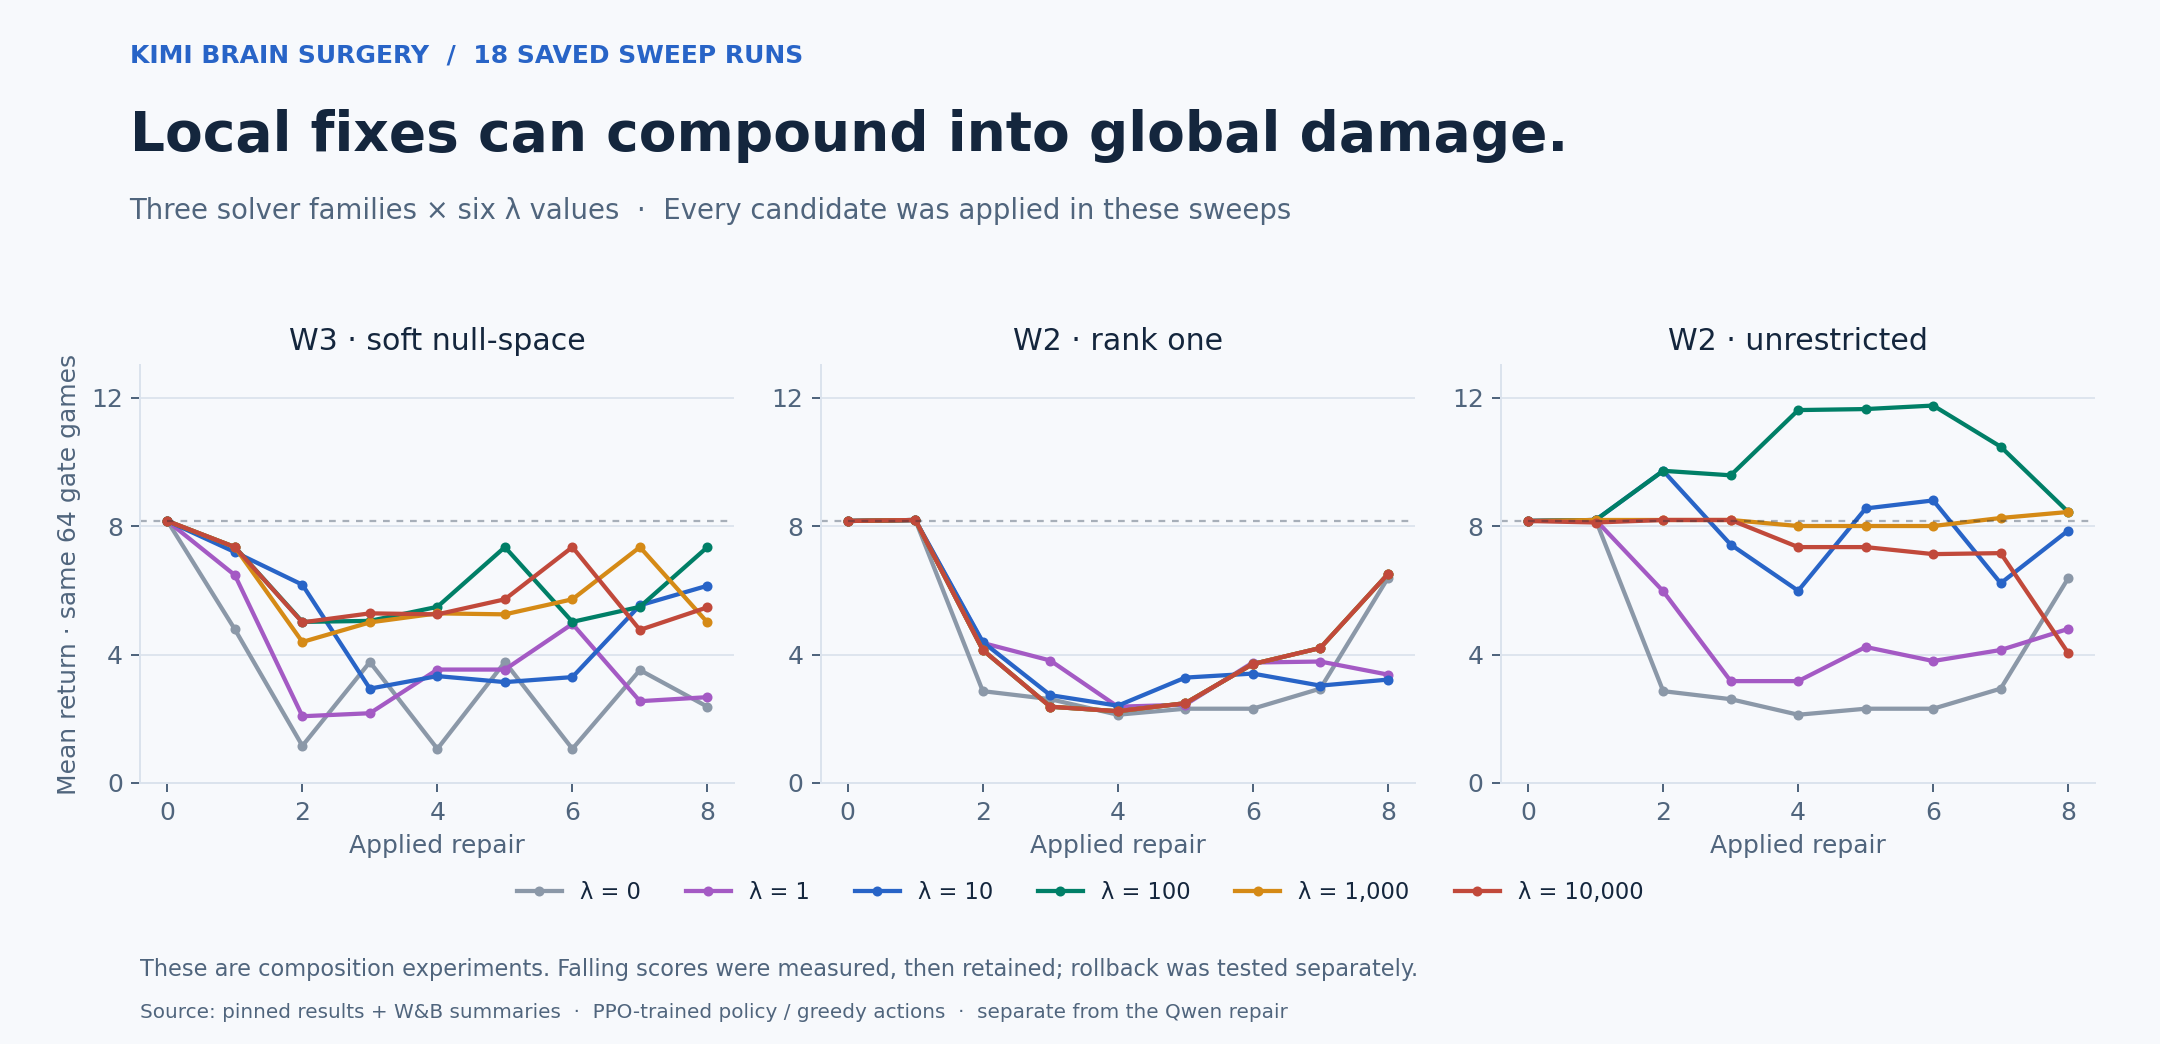
\includegraphics[width=\linewidth]{../assets/kimi-sweeps.png}
\end{center}
Each line starts at the same saved baseline gate mean and then follows eight
unconditionally applied repairs. A larger $\lambda$ changes the local
preservation metric; it does not guarantee a better trajectory-level outcome.
The axis is repair number, not training steps. There are no error bars because
these are exact recorded means on the same deterministic 64-game gate, not
independent replicate experiments.

\begin{center}
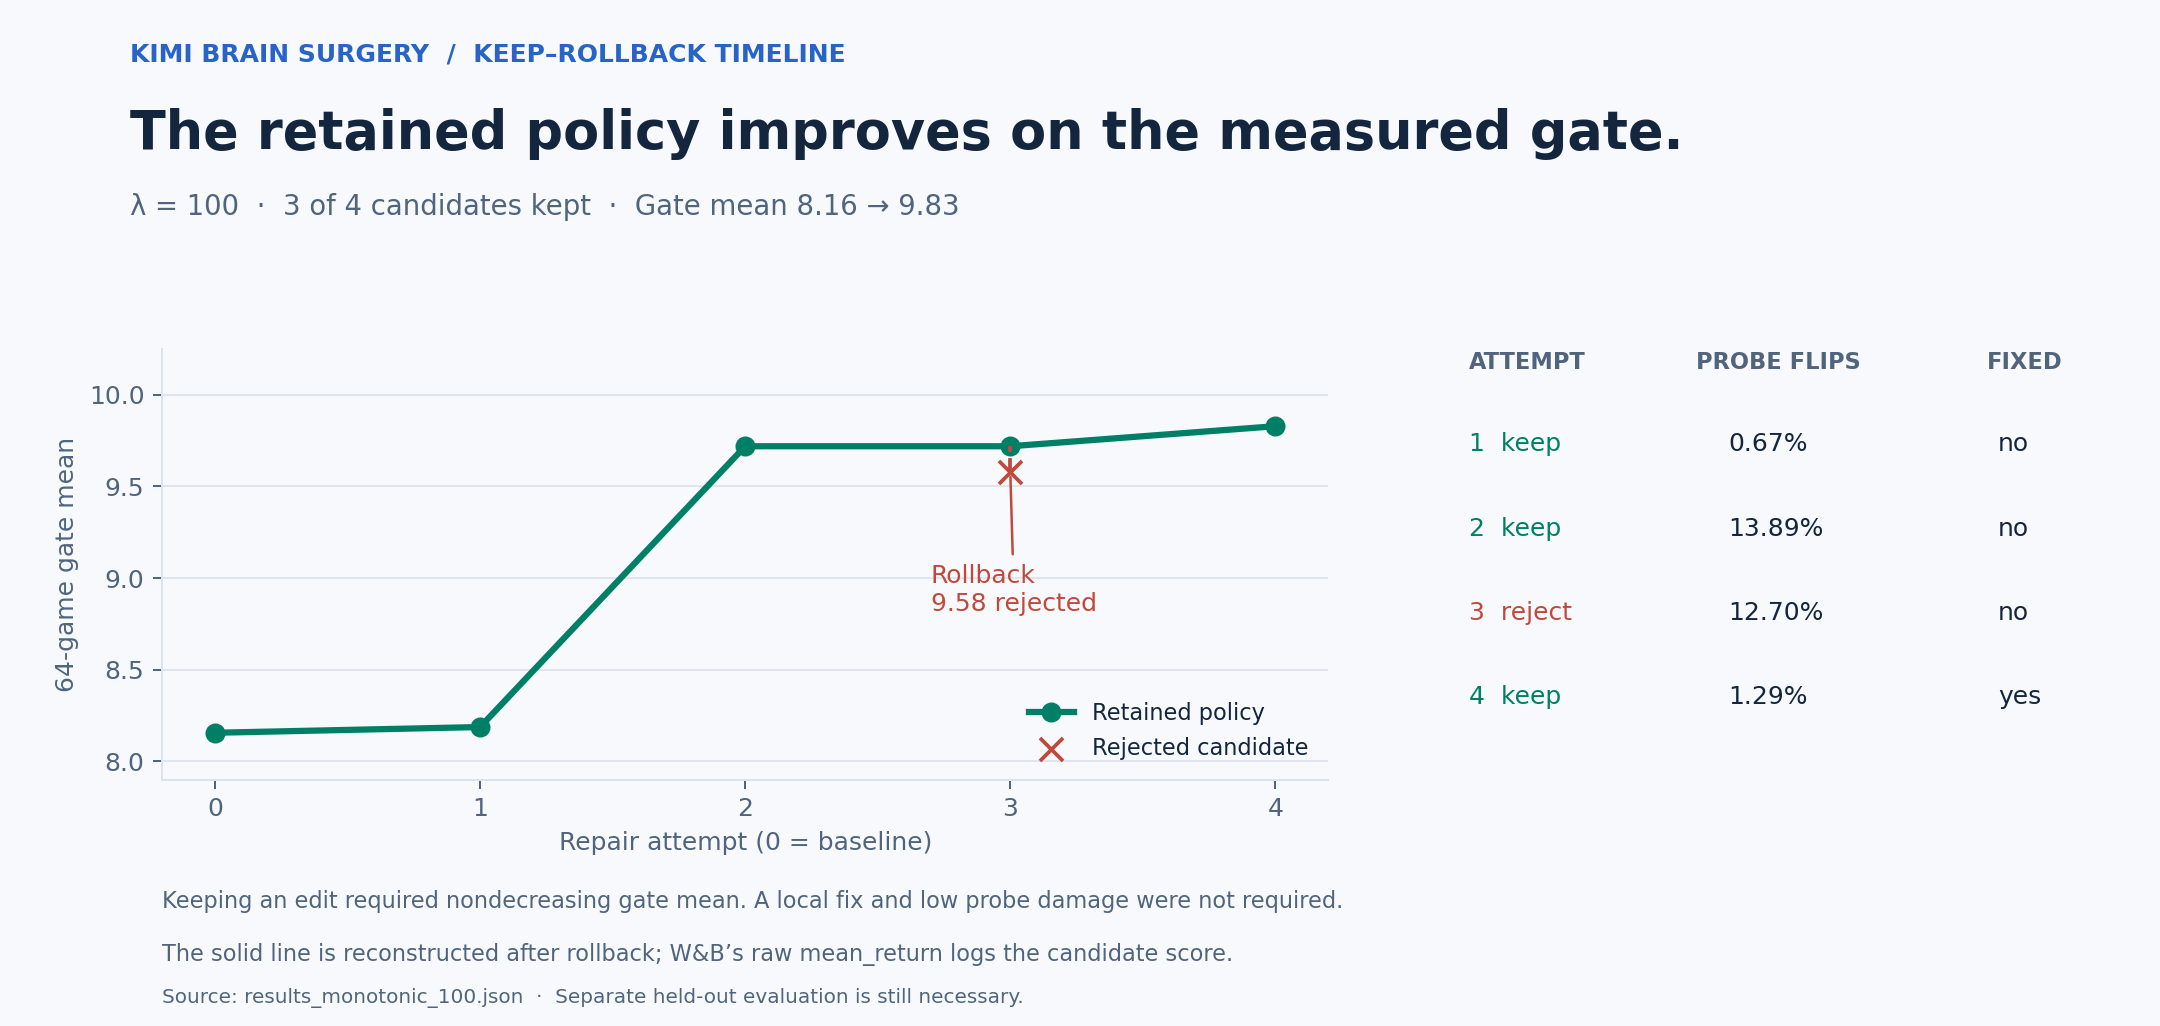
\includegraphics[width=\linewidth]{../assets/kimi-monotonic.png}
\end{center}
The solid incumbent line follows Equation~\eqref{eq:gate}; rejected candidate
scores remain visible. Probe damage and local repair status are separate
observations, not additional acceptance conditions in this run.

\small Plot inputs: the 18 \code{results_*_<lambda>.json} records and
\code{results_monotonic_100.json}. W\&B run identifiers and exact file hashes
are recorded in \code{results/kimi/provenance.json}.

\clearpage
\normalsize
\section{A precise interface for combining the two projects}
\textbf{Implemented here so far: two separate proposal mechanisms.}
KimiBrainSurgery uses analytic constrained solvers on a PPO-trained, greedily
evaluated policy. The completed Qwen trial in FailureIsAllYouNeed uses
tool-assisted scalar assignments on a handwritten policy with a planted
reversed-controls fault and sampled actions. Its three-parameter patch improved
average return on a separate gate and audit, but did not prevent the diagnostic
miss. Their scores should not be pooled or directly compared as a leaderboard.

\textbf{Proposed combination, not yet demonstrated.} Use an editor to examine
failure traces and propose a target action, layer, margin, and protected probe
set; call a numerical solver to produce an explicit candidate; then use one
independent verifier to test both the intended counterfactual and preservation.
Log the candidate and incumbent separately, preserve exact checkpoint hashes,
and deploy only accepted weights.

For a general differentiable policy, if $q(\theta)$ is a target logit difference,
the local equation is
\begin{equation}
 q(\theta+\delta)\simeq q(\theta)+J_f\delta,
 \qquad J_f=\nabla_\theta q(\theta)^{\mathsf T}.
\end{equation}
A prototype extension with several constraints is
\begin{equation}
 \min_\delta\;\tfrac12\delta^{\mathsf T}M\delta
 \quad\text{s.t.}\quad A\delta=r,
 \qquad
 \delta^*=M^{-1}A^{\mathsf T}
 (AM^{-1}A^{\mathsf T})^{-1}r,
 \label{eq:future}
\end{equation}
when $M\succ0$ and the rows of $A$ are independent. A pseudoinverse can handle
redundancy only with the appropriate feasibility checks. Inconsistent target
constraints require relaxing the problem. This multi-state formula is an
extension derived here, not an implemented result in the pinned Kimi code.

This explains the useful part of ``working backward'': start from a desired
change in behavior and solve for parameter changes that could realize it under
a specified preservation metric. The sensitivity map is usually many-to-one,
so this is not a unique inverse derivative. Nonlinear effects, changed future
state visitation, incomplete probes, and verifier blind spots remain.

\subsection*{What a combined acceptance rule would need to say}
A future protocol can require (i) rescue of a frozen counterfactual replay,
(ii) no unacceptable regressions on a protected suite, and (iii) a predefined
paired-performance criterion on reserved seeds. Those conditions must be
specified before selection; a reused practice gate is not an untouched audit.
An LLM's explanation of a repair is a hypothesis, not the acceptance test.

\subsection*{Attribution}
KimiBrainSurgery is HarleyCoops' parallel work built with Kimi. This methods
note translates that implementation; it does not attribute its numerical
results to the separate Qwen experiment. Both sit within a conceptual
replication effort inspired by Rikiya Takehi, Jayden Teoh, Alex Zhang, and Omar
Khattab's \href{https://rikiyat.github.io/blog/weight-space-programming/}{Sparks of Weight-Space Programming}.
See the \href{https://github.com/RikiyaT/lm_understand-logs/tree/main/exp1_which_game}{original experiment logs}.

\clearpage
\normalsize
\appendix
\section{Reproducibility and source map}
\begin{center}\small
\begin{tabular}{p{0.30\linewidth}p{0.61\linewidth}}
\toprule
Source file & Role in this document \\
\midrule
\code{failure_gym.py} & Network forward pass, landing predictors, reachability, diagnosis, naive readout edit. \\
\code{nullspace_gym.py} & Exact $W_3$ quadratic objective and symmetric column update. \\
\code{w2_gym.py} & Rank-one parameterization, diagonal metric, local corrections, and rollout gate. \\
\code{fullrank_gym.py} & Per-unit Gram matrices and block solves for unrestricted $W_2$. \\
\code{monotonic_gym.py} & Mean-return keep/rollback, unresolved failures, regression reports, best checkpoint. \\
\code{chase_unresolved.py} & Targeted layer/$\lambda$/margin grid. \\
\code{paired_eval.py} & Per-seed evaluation, paired bootstrap, and sign test. \\
\code{wandb_log.py} & Sweep curves, candidate metrics, checkpoint artifacts, paired tables. \\
\bottomrule
\end{tabular}\end{center}

All paths above resolve at the immutable source commit on page 1. The copied
results under \code{results/kimi/} are byte-identical to that snapshot.
\code{provenance.json} contains their SHA-256 hashes, checkpoint hashes,
source links, and a bounded W\&B run snapshot. Checkpoints remain in the
original project; this methods companion does not silently substitute or
republish Kimi's model artifacts.

\textbf{Rebuild the figures and numerical table} from the root of
FailureIsAllYouNeed:
\begin{verbatim}
python -m pip install -r requirements-figures.txt
python scripts/render_figures.py
python scripts/render_kimi_figures.py
python scripts/check_kimi_math.py
\end{verbatim}
The algebra checks exercise exact $W_3$ gap correction, diagonal and block
constraint solves, and the first-order $\tanh$ approximation. They do not rerun
the original repair experiment or certify unseen-game performance.

\textbf{Compile this document} with a standard LaTeX installation:
\begin{verbatim}
cd docs
pdflatex -interaction=nonstopmode -halt-on-error \
  kimi-parameter-repair.tex
pdflatex -interaction=nonstopmode -halt-on-error \
  kimi-parameter-repair.tex
\end{verbatim}
The second pass resolves equation and page references. Figures are rendered
from the saved per-attempt and per-seed data; generated plots do not smooth,
invent, or interpolate unseen evaluations.

\textbf{Evidence boundaries.} Logs and checkpoint hashes establish what was
saved. Source review establishes the implemented equations and selection rule.
Fresh paired rollouts establish measured behavior for a frozen candidate on a
particular distribution. None of these alone proves a unique causal mechanism,
universal non-regression, indefinite improvement, or transfer to Cree or Dakota.
\end{document}
